% !TeX spellcheck = en_US
\documentclass[authoryear]{elsarticle}
\usepackage{amsmath}
\usepackage{amssymb}
\usepackage{float}
\usepackage{graphicx}
\usepackage{subcaption}
\usepackage{changepage}
\usepackage{url}
\usepackage{xfrac}
\usepackage{booktabs}
\usepackage{rotating}
\usepackage{geometry}
%\usepackage{authblk}
\usepackage{xcolor}
%\usepackage{colortbl}
\usepackage{multirow}
%\usepackage{blindtext}
%\usepackage{mathtools}
%\usepackage{titlesec}
%\setcounter{secnumdepth}{4}
%\usepackage{wasysym}
%\usepackage{cleveref}
%\DeclarePairedDelimiter{\ceil}{\lceil}{\rceil}
\usepackage{lineno}
\linenumbers
\usepackage{setspace}
\doublespacing
\usepackage[flushleft]{threeparttable}
\usepackage[colorlinks,citecolor=blue,urlcolor=blue]{hyperref} 
%\usepackage{apacite}
\bibliographystyle{elsarticle-harv}

\makeatletter
\def\ps@pprintTitle{%
	\let\@oddhead\@empty
	\let\@evenhead\@empty
	\def\@oddfoot{\centerline{\thepage}}%
	\let\@evenfoot\@oddfoot}
\makeatother

% Remove abstract section
\makeatletter
\long\def\pprintMaketitle{\clearpage
	\iflongmktitle\if@twocolumn\let\columnwidth=\textwidth\fi\fi
	\resetTitleCounters
	\def\baselinestretch{1}%
	\printFirstPageNotes
	\begin{center}%
		\thispagestyle{pprintTitle}%
		\def\baselinestretch{1}%
		\Large\@title\par\vskip18pt
		\normalsize\elsauthors\par\vskip10pt
		\footnotesize\itshape\elsaddress\par\vskip36pt
		% \hrule\vskip12pt
		% \ifvoid\absbox\else\unvbox\absbox\par\vskip10pt\fi
		% \ifvoid\keybox\else\unvbox\keybox\par\vskip10pt\fi
		% \hrule\vskip12pt
	\end{center}%
	\gdef\thefootnote{\arabic{footnote}}%
}
\makeatother

\begin{document}
	\begin{frontmatter}
		\title{
			%		Anthropocentric uses of phosphorus: flows quantification and potential for recycling in Ontario
			%	Mapping phosphorus flows in the economic sectors of Ontario and assessing recovery and recycling potential
			Supplementary Information: \\ Phosphorus in Ontario's economic sectors: mapping flows and assessing recovery and recycling potential
		}
		
		%% Group authors per affiliation:
		\author[ULaval]{Université Laval team\corref{mycorrespondingauthor}}
		\cortext[mycorrespondingauthor]{Corresponding author}
		\ead{edgar.martin-hernandez.1@ulaval.ca}
		%	%\fntext[myfootnote]{Since 1880.}
		\author[McGill]{McGill University team}
		\author[Waterloo]{University of Waterloo team}
		
		\address[ULaval]{Université Laval}
		\address[McGill]{McGill University}
		\address[Waterloo]{University of Waterloo}
		
%		\begin{abstract}
%			
%		\end{abstract}
		%	
		%	\begin{keyword}
		%		Quantifying P flows in Ontario's agricultural sector 
		%	\end{keyword}
	\end{frontmatter}
	
	\tableofcontents
	
\section{Distribution of CAFOs size in regions of the the Great Lakes area}
The size distribution of Ontario's CAFOs is not reported by public databases, but the number of animals is aggreggated at Census Division level REF, REF. As an approximation, the size distribution of CAFOs of other regions in the vicinity of the Great Lakes area reporting the size of CAFOs is calculated and extrapolated to the province of Ontario. The size distribution of CAFOs is determined for the US states of Ohio REF, Pennsylvania REF, Indiana REF, Michigan REF, and Wisconsin REF. The distribution of CAFOs size has been fit to a truncated normal distribution REF INCLUDE EQUATION, since the possible size of livestock facilities is bounded between 300 animal units for being considered as an intensive livestock production facility REF, and 10,000 animal units in order to remove extra-large CAFOs that are outliers in the size distribution, avoiding excessive long tails distorting the distributions. Figure \ref{fig:CAFOsSizeDist} represent the distribution of CAFOs using the kernel density estimation (KDE) REF, and the fitting parameters for the truncated normal distribution for each evaluated region.
\begin{figure}[H]
	\centering
	%	\begin{subfigure}[t]{0.5\linewidth}
	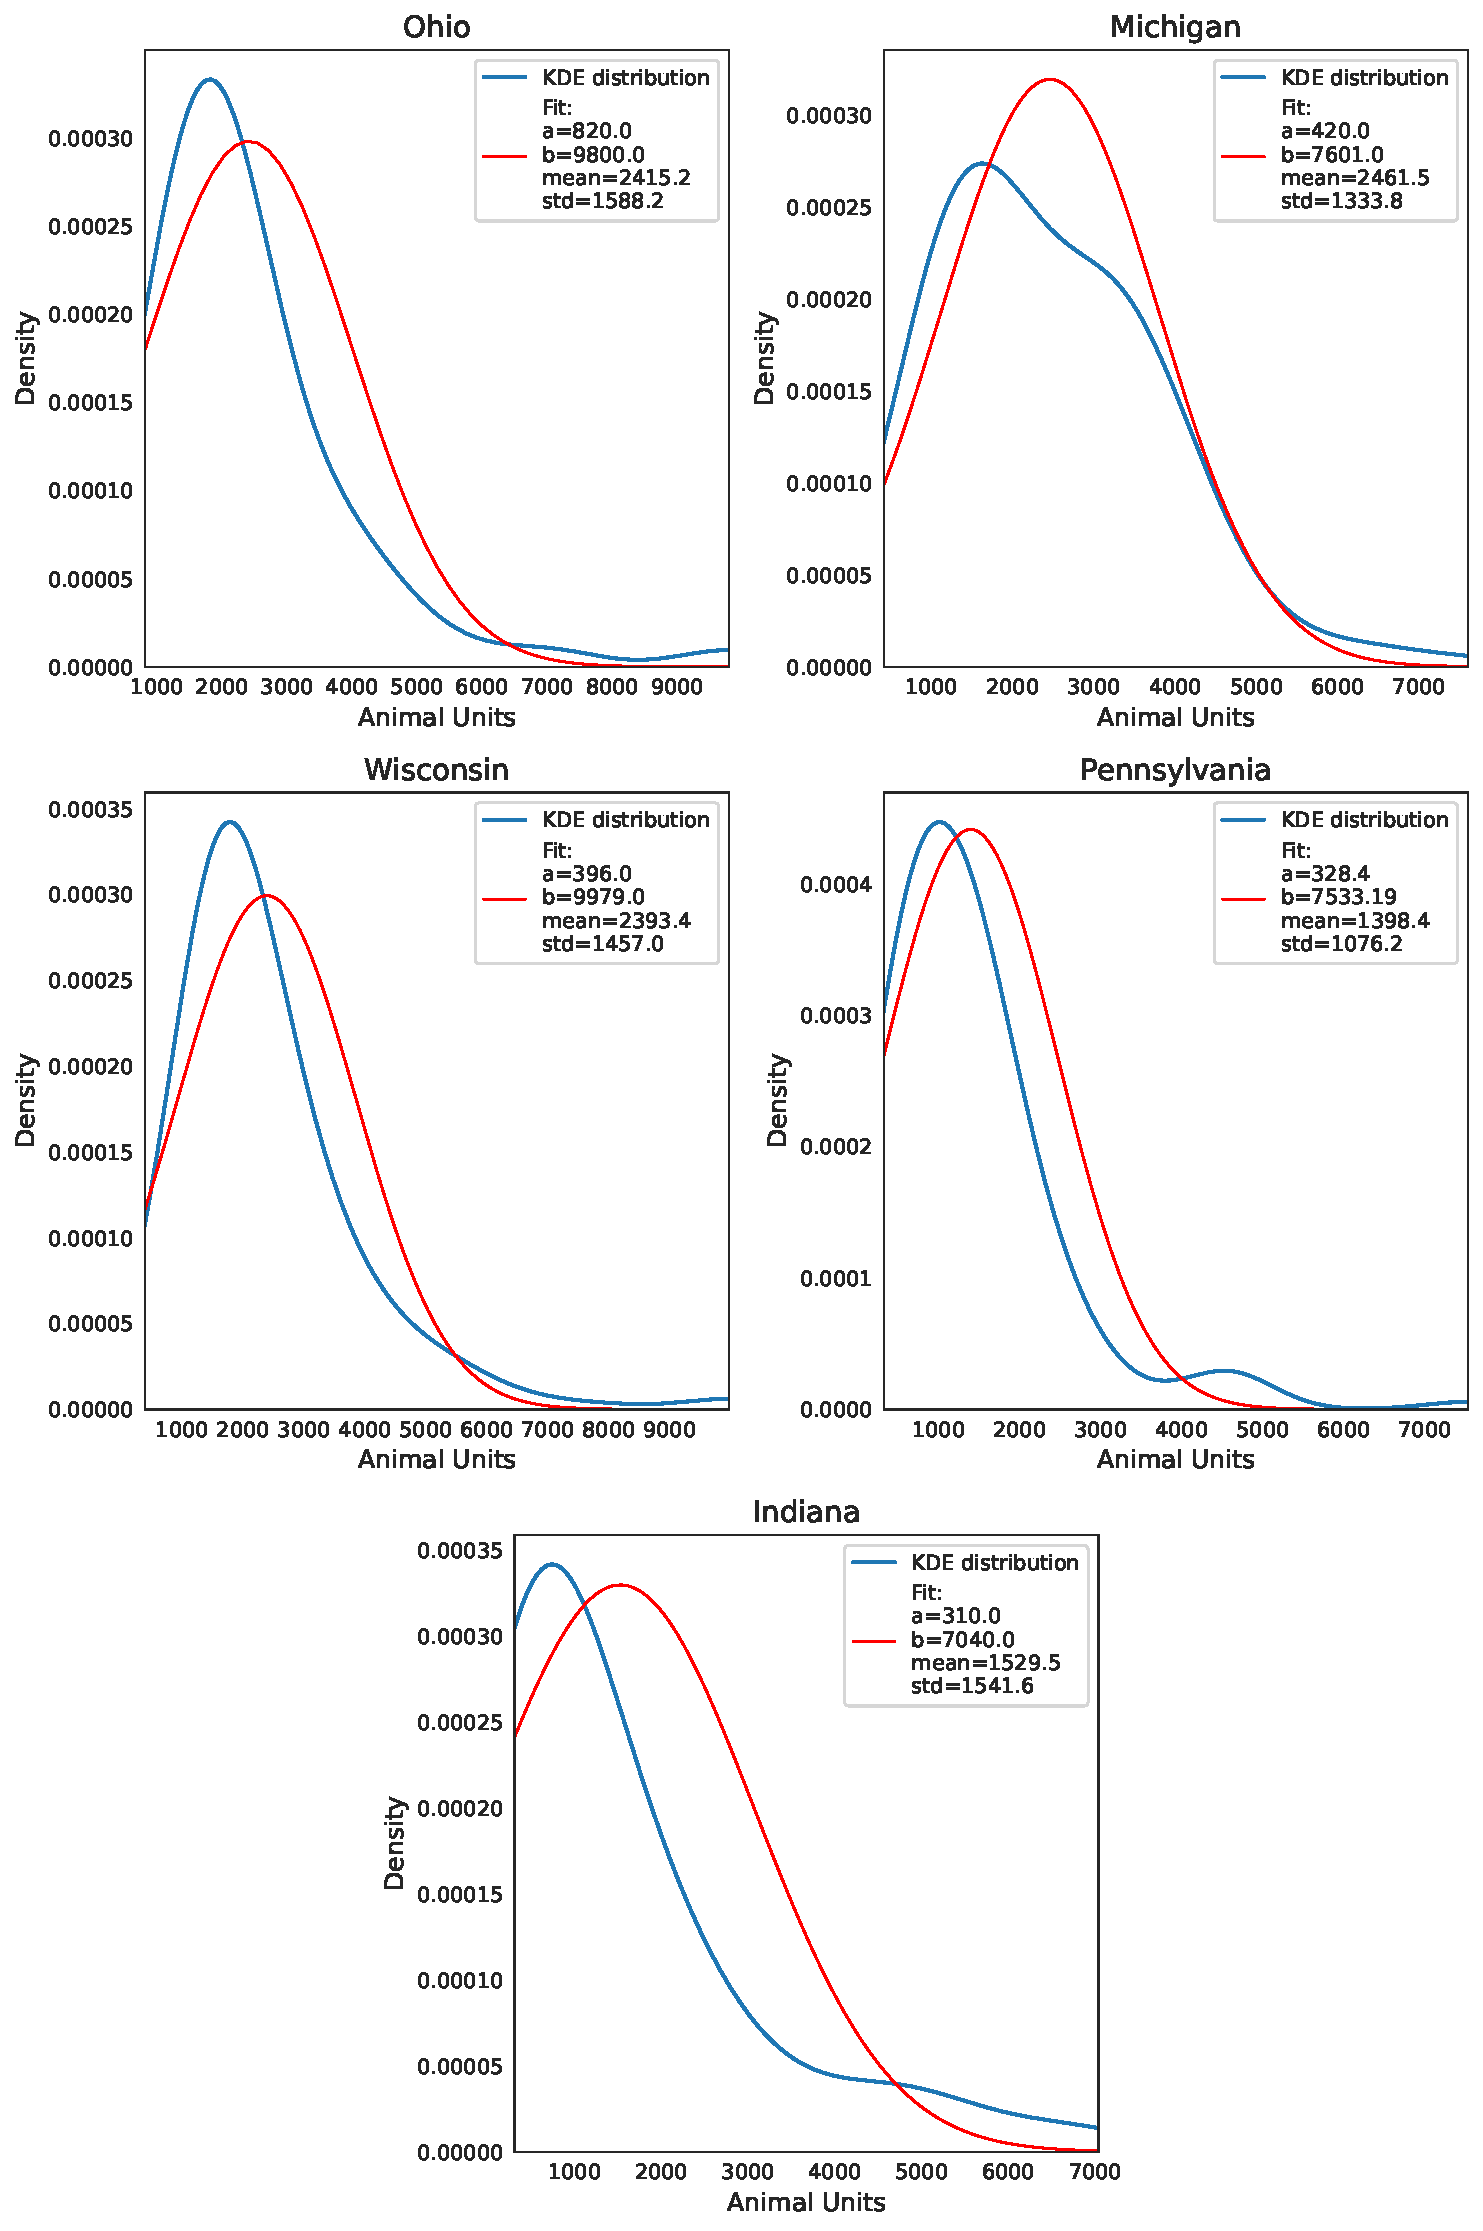
\includegraphics[width=0.81\linewidth, trim={0cm 0cm 0cm 0cm},clip]{SupMat_Figures/CAFOs_Size_Distribution} 
	\caption{Distribution of CAFOs size in regions of the the Great Lakes area.}
	\label{fig:CAFOsSizeDist}
\end{figure}
	
%\bibliographystyle{apacite}
%\bibliographystyle{ieee}
\bibliography{references}
	
\end{document}